% !TEX root = ../../../main.tex
% 所属：第一部分：单变量分析学 / 第1章：实数理论——从Peano公理到实数的连续性
% 节：1.9 映射，有限集和可数集
% 正文按原文件顺序保存；由 ../chapter1.tex 调用。
\section{映射，有限集和可数集}
\begin{definition}
	考虑两个集 $A$ 和 $B$ ，它们的元素可以是任何东西．
	
	假定对于 $A$的每个元素 $x$ ，按照某种方式，与集 $B$ 的一个元素联系着，这个元素记作 $f(x)$ ；那么，就说 $f$ 是从 $A$ 到 $B$ 的一个函数（或将 $A$ 映入 $B$ 内的一个映射）．集 $A$ 叫做 $f$ 的定义域（或者说 $f$ 定义在 $A$ 上），而元素 $f(x)$ 叫做 $f$ 的值．$f$ 的一切值的集叫做 $f$ 的值域．
	
	定义域$A$,值域$B$,这种关系(法则)$f$,三者的整体，我们称为一个函数.
	
\end{definition}
\begin{definition}
	设 $A$ 和 $B$ 是两个集，$f$ 是 $A$ 到 $B$ 内的一个映射．
	
	如果 $E \subset A$ ，对于一切 $x \in E$ ，元素 $f(x)$ 所成的集定义为 $f(E)$ .我们称 $f(E)$ 为 $E$ 在 $f$ 之下的象．
	
	按这个记法来说，$f(A)$ 就是 $f$ 的值域．显然 $f(A) \subset B$ ．如果 $f(A)=B$ ，就说 $f$ 将 $A$ 映满 $B$ .
	
	$E \subset B$ 时，$f^{-1}(E)$ 表示一切合于 $f(x) \in E$ 的 $x \in A$ 所成的集．称 $f^{-1}(E)$ 为 $E$ 在 $f$ 之下的逆象. $y \in E$ 时，$f^{-1}(E)$ 是 $A$ 中一切合于 $f(x)=y$ 的元素 $x$ 所成的集．
	
	如果 $f^{-1}(y)$ 对于每个 $y \in B$ 至多含有 $A$ 中的一个元素，那么就称 $f$ 是 $A$ 到 $B$内的 $1-1$（一对一的）映射．这句话也可以表述如下：如果对于 $x_1 \in A, x_2 \in A$ ，当 $x_1 \neq x_2$ 时，$f\left(x_1\right) \neq f\left(x_2\right)$ ，那么 $f$ 就是 $A$ 到 $B$ 内的一个 $1-1$ 映射．
	
	
	$\left(x_1 \neq x_2\right.$ 表示 $x_1$ 和 $x_2$ 是不同的元素；否则就记作 $x_1=x_2$ .）
\end{definition}
\begin{definition}
	若存在A到B上的$1-1$映射，A,B之间就存在一个 等价关系.
\end{definition}
\begin{definition}
	对于任意正整数 $n$ ，令 $J_n$ 表示 $1,2, \cdots, n$ 所成的集，令 $\Z_+$ 表示全体正整数所成的集．设 $A$ 是任意一个集．我们说
	\begin{enumerate}
		\item $A$ 是有限的，如果对于某个 $n, A \sim J_n$（空集也认为是有限集）
		\item $A$ 是无限的，如果 $A$ 不是有限的．
		\item $A$ 是可数的，如果 $A \sim \Z_+$
		\item $A$ 是不可数的，如果 $A$ 既不是有限的，也不是可数的．
		\item $A$ 是至多可数的，如果 $A$ 或为有限或为可数的．
	\end{enumerate}
	
\end{definition}
\begin{definition}
	定义在一切正整数的集 $\Z_+$ 上的函数叫做一个序列，如果对于 $n \in \Z_+, f(n)=x_n$ ，习惯上就把序列 $f$ 用符号 $\left\{x_n\right\}$ 来表示，或者用 $x_1, x_2, x_3, \cdots$来表示．$f$ 的值，即元素 $x_n$ ,叫做这个序列的项．设 $A$ 是一个集并且对一切 $n \in \Z_+$ ， $x_n \in A$ ，那么 $\left\{x_n\right\}$ 就叫做 $A$ 里的一个序列，或者叫做 $A$ 的元素的一个序列．
	
	
\end{definition}
注意，一个序列的项 $x_1, x_2, x_3, \cdots$ 不一定各不相同
\begin{proposition}
	可数集 $A$ 的每个无限子集也是可数集．
\end{proposition}

\begin{proof}
	设 $E \subset A$ 并且 $E$ 是无限集．把 $A$ 的元素 $x$ 排成一个不同元素的序列 $\left\{x_n\right\}$ .按以下方式作序列 $\left\{n_k\right\}$ ：
	
	令 $n_1$ 是使 $x_{n_1} \in E$ 的最小正整数．当 $n_1, \cdots, n_{k-1}(k=2,3,4, \cdots)$ 选定以后，令 $n_k$ 是大于 $n_{k-1}$ 并且使 $x_{n_k} \in E$ 的最小正整数．
	
	令 $f(k)=x_{n_k}(k=1,2,3, \cdots)$ ，我们便得到了 $E$ 和 $\Z_+$ 之间的一个 $1-1$ 对应．
\end{proof}
\begin{proposition}
		设 $\left\{E_n\right\} n=1,2,3, \cdots$ 是可数集组成的序列，令
	
	$$
	S=\bigcup_{n=1}^{\infty} E_n,
	$$
	
	
	那么 $S$ 是可数的．\label{uniofconset}
\end{proposition}

\begin{proof}
	把每个集 $ E_n$   排成一个序列 $\left\{x_{n _k}\right\}, k=1,2,3, \cdots $，而来考虑无限阵列 
	\begin{center}
		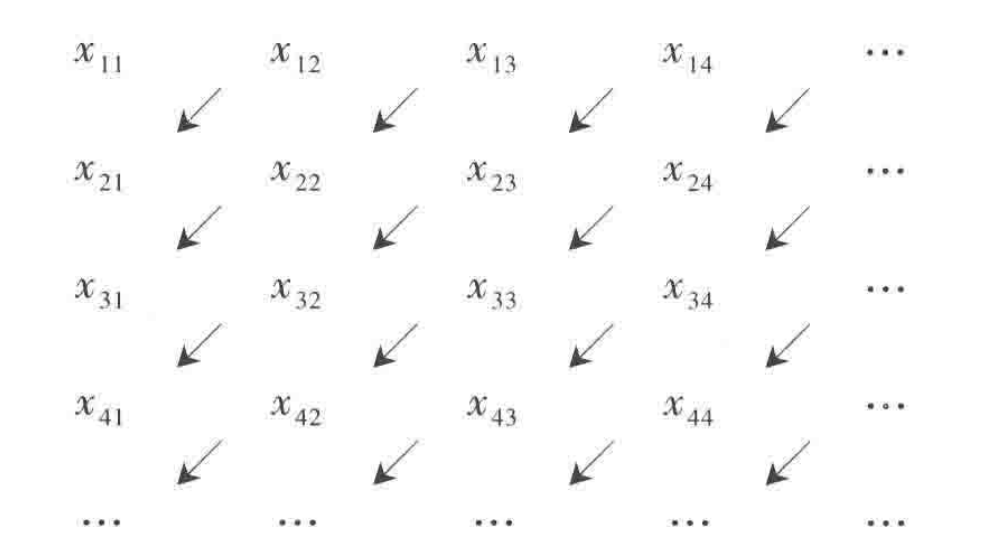
\includegraphics[width=0.7\linewidth]{figure/C1/8e9c0c930834b91d997911bb6ae34b5a}
	\end{center}
	

	把所有的元素排列成
	
	$$
	x_{11}, x_{12}, x_{21}, x_{13}, x_{22}, x_{31}, x_{14}, x_{23}, x_{32}, x_{41}, \cdots,
	$$
	这些集 $E_n$ 的任何两个如果有公共元素，那么这些公共元素将在上面的排列中不止出现一次.因此一切正整数的集里有一个子集 $T\subset\Z_+$ 使得 $S \sim T$ ，这就证明了 $S$ 是至多可数的.因为 $E_1 \subset S$ ，而 $E_1$ 是无限的，所以 $S$ 也是无限的，从而是可数的.
	
\end{proof}
\begin{corollary}\label{1.9.8}
	假定 $A$ 是至多可数的，并且对应于每个 $\alpha \in A$ 的 $B_\alpha$ 是至多可数
	的．令
	
	$$
	T=\bigcup_{\alpha \in A} B_\alpha
	$$
	
	
	那么 $T$ 是至多可数的．
\end{corollary}
$T$是\ref{uniofconset}中的$S$的一个子集.
\begin{proposition}
	\label{couofdes}
	$A_i$ 是可数集，$B_n=A_1 \times \cdots \times A_n$ 那么 $B_n$ 是可数的.
	
	换言之，可数集的有限次 Descartes 积是可数的
\end{proposition}

\begin{proof}
	$n=2$ 时 $ B_2=A_1 \times A_2=\left\{\left(x_1, x_2\right): x_1 \in A_1, x_2 \in A_2\right\}$
	
	令 $a_{i j}=\left(x_{1 i} , x_{2 j}\right)$ 由\ref{1.9.8}中的构造. $B_2$ 可数
	
	设 $B_{k-1}$ 可数
	
	$$
	B_k=A_1 \times \cdots A_{k-1} \times A_k=B_{k-1} \times A_k
	$$
	可数.
\end{proof}

\begin{remark}
	可数集的可数 次 Descartes 积不是可数的，使用下一节的定义，这个集合与 $\mathbb{R}$ 等势.
\end{remark}

下面我们考察一些集合的可数性.
\begin{proposition}
		$\Z,\Q$可数，$\R$不可数.
\end{proposition}

\begin{proof}
	对$\Z$ $f(n)=\left\{\begin{array}{cc}\dfrac{n}{2} & n \text { 是偶数 } \\ -\dfrac{n-1}{2} & n \text { 是奇数 }\end{array}\right.$
	
	对$\Q$由\ref{couofdes}可得
	
	对 $\mathbb{R}$ ,只需证 $(0,1)$ 内的所有实数不可数.
	
	如若不然，将所有 $(0,1)$ 内的实数用十进小数列出
	
	$$
	\begin{aligned}
		& r_1=0 . \overline{a_{11} a_{12} a_{13} a_{14}} \\
		& r_2=0 . \overline{a_{21} a_{22} a_{23} a_{24}} \cdots \\
		& r_3=0 . \overline{a_{31} a_{32} a_{33} a_{34}} \cdots \\
		& r_4=0 . \overline{a_{41} a_{42} a_{43} a_{44}} \cdots
	\end{aligned}
	$$
	
	
	构造 $b=0 . \overline{b_1 b_2 b_3 b_4} \cdots$ 使得 $b_1 \neq a_{11}, b_2 \neq a_{22}, b_3 \neq a_{33} \cdots$
	比如记 
	
	$\ b_n=\left[\begin{array}{ll}1 & \text { 若 }a_{n n} \neq 1 \\ 2 &\text { 若 } a_{n n}=1\end{array}\right.$
	
	$b$这个实数不在列表当中 ，矛盾，故不可数.
\end{proof}


\begin{lemma}(像-原像引理)
	设 \( f: X \to Y \) 是两个集合 \( X \) 和 \( Y \) 之间的映射，则以下命题成立：
	
	\begin{enumerate}
		\item[(0)]
		\begin{tabular}{ll}
			(a) & \( X = f^{-1}(Y) \) \\
			(b) & \( \varnothing  = f^{-1}(\varnothing ) \)
		\end{tabular}
		
		\item[(1)]
		\begin{tabular}{ll}
			(a) & 对于任意子集 \( U \subset X \)，有 \( U \subset f^{-1}(f(U)) \) \\
			(b) & 进一步，如果 \( f \) 是单射，则有 \( U = f^{-1}(f(U)) \)
		\end{tabular}
		
		\item[(2)]
		\begin{tabular}{ll}
			(a) & 对于任意子集 \( V \subset Y \)，有 \( V \supset f(f^{-1}(V)) \) \\
			(b) & 进一步，如果 \( f \) 是满射，则有 \( V = f(f^{-1}(V)) \)
		\end{tabular}
		
		\item[(3)] 对于 \( X \) 的任意一族子集 \(\{U_i\}_{i \in I}\)，有
		\[ f\left(\bigcup_{i \in I} U_i\right) = \bigcup_{i \in I} f(U_i) \]
		
		\item[(4)] 对于 \( X \) 的任意一族子集 \(\{U_i\}_{i \in I}\)，有
		\[ f\left(\bigcap_{i \in I} U_i\right) \subseteq \bigcap_{i \in I} f(U_i) \]
		
		\item[(5)]
		\begin{tabular}{ll}
			(a) & 对于任意子集 \( U \subset X \)，有 \( f(X \setminus U) \supset f(X) \setminus f(U) \) \\
			(b) & 进一步，如果 \( f^{-1}(f(U)) = U \)，则有 \( f(X \setminus U) = f(X) \setminus f(U) \)
		\end{tabular}
		
		\item[(6)] 对于 \( Y \) 的任意一族子集 \(\{V_i\}_{i \in I}\)，有
		\[ f^{-1}\left(\bigcup_{i \in I} V_i\right) = \bigcup_{i \in I} f^{-1}(V_i) \]
		
		\item[(7)] 对于 \( Y \) 的任意一族子集 \(\{V_i\}_{i \in I}\)，有
		\[ f^{-1}\left(\bigcap_{i \in I} V_i\right) = \bigcap_{i \in I} f^{-1}(V_i) \]
		
		\item[(8)] 对于任意子集 \( V \subset Y \)，有
		\[ f^{-1}(Y \setminus V) = X \setminus f^{-1}(V) \]
	\end{enumerate}
\end{lemma}

\begin{proof}
	\begin{enumerate}
		\item[(0)]
		\begin{enumerate}
			\item[(a)] 对于任意 \( x \in X \)，有 \( f(x) \in Y \)，因此 \( x \in f^{-1}(Y) \)，所以 \( X \subseteq f^{-1}(Y) \)。又因为 \( f^{-1}(Y) \subseteq X \)，所以 \( X = f^{-1}(Y) \)。
			
			\item[(b)] 因为 \( f^{-1}(\emptyset) = \{ x \in X \mid f(x) \in \emptyset \} = \emptyset \)，所以 \( \emptyset = f^{-1}(\emptyset) \)。 \end{enumerate}
		
		\item[(1)]
		\begin{enumerate}
			\item[(a)] 对于任意 \( x \in U \)，有 \( f(x) \in f(U) \)，因此 \( x \in f^{-1}(f(U)) \)，所以 \( U \subseteq f^{-1}(f(U)) \)。
			
			\item[(b)] 如果 \( f \) 是单射，且 \( x \in f^{-1}(f(U)) \)，则 \( f(x) \in f(U) \)，即存在 \( u \in U \) 使得 \( f(x) = f(u) \)。由于 \( f \) 是单射，所以 \( x = u \in U \)，因此 \( f^{-1}(f(U)) \subseteq U \)。结合 (1a) 可得 \( U = f^{-1}(f(U)) \)。 \end{enumerate}
		
		\item[(2)]
		\begin{enumerate}
			\item[(a)] 对于任意 \( y \in f(f^{-1}(V)) \)，存在 \( x \in f^{-1}(V) \) 使得 \( f(x) = y \)。根据定义，\( f(x) \in V \)，所以 \( y \in V \)，因此 \( f(f^{-1}(V)) \subseteq V \)。
			
			\item[(b)] 如果 \( f \) 是满射，对于任意 \( y \in V \)，存在 \( x \in X \) 使得 \( f(x) = y \)。因为 \( y \in V \)，所以 \( x \in f^{-1}(V) \)，因此 \( y \in f(f^{-1}(V)) \)，所以 \( V \subseteq f(f^{-1}(V)) \)。结合 (2a) 可得 \( V = f(f^{-1}(V)) \)。 \end{enumerate}
		
		\item[(3)] 对于任意 \( y \in f\left(\bigcup_{i \in I} U_i\right) \)，存在 \( x \in \bigcup_{i \in I} U_i \) 使得 \( f(x) = y \)。这意味着存在 \( i \in I \) 使得 \( x \in U_i \)，因此 \( y \in f(U_i) \)，所以 \( y \in \bigcup_{i \in I} f(U_i) \)。反之，对于任意 \( y \in \bigcup_{i \in I} f(U_i) \)，存在 \( i \in I \) 使得 \( y \in f(U_i) \)，因此存在 \( x \in U_i \) 使得 \( f(x) = y \)，所以 \( y \in f\left(\bigcup_{i \in I} U_i\right) \)。因此等式成立。
		
		\item[(4)] 对于任意 \( y \in f\left(\bigcap_{i \in I} U_i\right) \)，存在 \( x \in \bigcap_{i \in I} U_i \) 使得 \( f(x) = y \)。对于任意 \( i \in I \)，有 \( x \in U_i \)，因此 \( y \in f(U_i) \)，所以 \( y \in \bigcap_{i \in I} f(U_i) \)。
		
		\item[(5)]
		\begin{enumerate}
			\item[(a)] 对于任意 \( y \in f(X) \setminus f(U) \)，存在 \( x \in X \) 使得 \( f(x) = y \) 且 \( x \notin U \)，即 \( x \in X \setminus U \)，因此 \( y \in f(X \setminus U) \)。
			
			\item[(b)] 如果 \( f^{-1}(f(U)) = U \)，对于任意 \( y \in f(X) \setminus f(U) \)，假设 \( y \in f(U) \)，则存在 \( x \in U \) 使得 \( f(x) = y \)，这意味着 \( x \in f^{-1}(f(U)) = U \)，矛盾。因此 \( f(X \setminus U) \subseteq f(X) \setminus f(U) \)。结合 (5a) 可得 \( f(X \setminus U) = f(X) \setminus f(U) \)。 \end{enumerate}
		
		\item[(6)] 对于任意 \( x \in f^{-1}\left(\bigcup_{i \in I} V_i\right) \)，有 \( f(x) \in \bigcup_{i \in I} V_i \)，即存在 \( i \in I \) 使得 \( f(x) \in V_i \)，因此 \( x \in f^{-1}(V_i) \)，所以 \( x \in \bigcup_{i \in I} f^{-1}(V_i) \)。反之亦然，因此等式成立。
		
		\item[(7)] 对于任意 \( x \in f^{-1}\left(\bigcap_{i \in I} V_i\right) \)，对于任意 \( i \in I \)，有 \( f(x) \in V_i \)，因此 \( x \in f^{-1}(V_i) \)，所以 \( x \in \bigcap_{i \in I} f^{-1}(V_i) \)。反之亦然，因此等式成立。
		
		\item[(8)] 对于任意 \( x \in f^{-1}(Y \setminus V) \)，有 \( f(x) \in Y \setminus V \)，即 \( f(x) \notin V \)，因此 \( x \notin f^{-1}(V) \)，所以 \( x \in X \setminus f^{-1}(V) \)。反之亦然，因此等式成立。
	\end{enumerate}
\end{proof}
现在，我们用集合的方式，对映射再此定义，同时我们可以定义出二元运算的集合论形式.
\begin{definition}指派法则是两个集合的笛卡儿积 $C \times D$ 的一个子集 $r$，该子集满足这样的条件：$C$ 的每一个元素最多是 $r$ 中一个有序偶对的第一个坐标.
	
	这样，$C \times D$ 的一个子集 $r$ 如果满足
	
	$$
	\left[(c, d) \in r \text { 并且 }\left(c, d^{\prime}\right) \in r\right] \Longrightarrow\left[d=d^{\prime}\right] \text {, }
	$$
	则成为一个指派法则．我们可以将 $r$ 设想成一种指派方法，为 $C$ 的元素 $c$ 配置 $D$ 的满足 $(c, d) \in r$的元素 $d$ .
	
	对于一个指派法则 $r$ ，其定义域是由 $r$ 的元素的所有第一个坐标组成的 $C$ 的子集，其值域是由 $r$ 的元素的所有第二个坐标组成的 $D$ 的子集，即
	
	$r$ 的定义域 $=\{c $: 存在 $d \in D$ ，使得 $(c, d) \in r\}$ ，
	
	$r$ 的值域 $=\{d $ :存在 $c \in C$ ，使得 $(c, d) \in r\}$ ．
	
	函数$f$是指派法则$r$,与其定义域和值域三者组成的整体.
\end{definition}
\begin{definition}
	集合  $A $ 中的一个二元运算是将  $A \times A$ 映到  $A  $中的一个函数$  f $
\end{definition}
这样无论是整个实数的体系，还是函数的定义，或者是加减乘除的二元运算，都建立在公理化的集合论之上.
